\begin{frame}
  \frametitle{Outline}

  \tableofcontents
\end{frame}



\begin{frame}
	\frametitle{Planning the mission of Philae on the comet 67P \mycite{SimoninEtAl15}}

	\begin{columns}
	\begin{column}{0.4\textwidth}
		
			\begin{itemize}
				\item Jobs: Scientific experiments
				\item Resources:
				\begin{itemize}
					\item \memph{Batteries}: threshold on the instant energy consumption
					\only<2->{
					\begin{itemize}
						\item Nested cumulative constraints
					\end{itemize}
					}
					\item \memph{Memory}: experiments produce data and transfers are possible only when Rosetta is visible
					\only<2->{
					\begin{itemize}
						\item \memph{Memory / transfer channel resources (?)}
					\end{itemize}
					}
				\end{itemize}
				% \item Maximise the lifespan of the batterie
			\end{itemize}

	\end{column}
	\begin{column}{0.6\textwidth}  %%<--- here
		\begin{center}

	     \includegraphics[width=0.75\textwidth]{im/philaeexp.jpg}
			 
			 \includegraphics[width=0.45\textwidth]{im/ampoule.jpg}
			 \includegraphics[width=0.45\textwidth]{im/floppydisk.png}
			 
		\end{center}
	\end{column}
	\end{columns}
	
	% \ShowPutAtGrid
	
	\PutAt<2->{(6.5cm,7cm)}{
	\FlashyBox[font=\footnotesize]{Cumulative}
	}
	
	\PutAt<2->{(10cm,7cm)}{
	\FlashyBox[font=\footnotesize]{~~~??~~~}
	}
	

\end{frame}



\begin{frame}[fragile]
	\frametitle{Command and Data Management Subsystem} 
	
	\uncover<2->{
	% \begin{itemize}
		\hfill \textcolor{white}{()}\only<2>{(\memph{non-visibility})}\only<3->{(\memph{visibility})}
	% \end{itemize}
	}
	
% Define module styles
\tikzstyle{hub} = [diamond, draw=DarkBlue, top color=Teal!50!black, bottom color=Teal, drop shadow, text=white, 
    text width=4.5em, text badly centered, node distance=2.8cm, inner sep=0pt]
\tikzstyle{module} = [rectangle, draw=DarkBlue, top color=Teal!50, bottom color=Teal, drop shadow, 
    text width=4.5em, text centered, rounded corners, minimum height=3.8em]
\tikzstyle{line} = [draw, very thick, -latex, shorten >=2pt,shorten <=2pt]
\tikzstyle{satellite} = [ellipse, draw=FireBrick, top color=OrangeRed!30, bottom color=Red!70!black, node distance=.9cm,
    minimum height=2em, drop shadow]
    
		\begin{center}
\begin{tikzpicture}[scale=.75]
	
	\tikzset{prio/.style={single arrow,draw=FireBrick,top color=OrangeRed!30, bottom color=Red!70!black}}
	
    % Place nodes
		
		\node [hub] (cdms) at (0,0) {CDMS};
		
		\uncover<2-> {
				\node [prio, above right =.7cm and 2.4cm of cdms, rotate=270, minimum height=3.6cm] {~~prio~~~~~~~~-rity};  
		}
		
		\invisible<2> {
	 	\node [above left = 1.6cm and -.3cm of cdms] (rosetta) {\includegraphics[width=5cm]{im/rosetta.png}};
		}
		
		\node [module, left = 1.5cm of cdms] (memory) {Mass Memory};
		\node [satellite, above right = 3.6cm and 4cm of cdms] (exp1) {{\small Exp. 1}};
		\node [module, minimum height=2em, below left = .6cm and 0.25cm of exp1] (mem1) {{\small Mem. 1}};
		\node [satellite, below = 1.5cm of exp1] (exp2) {{\small Exp. 2}};
		\node [module, minimum height=2em, below left = .6cm and 0.25cm of exp2] (mem2) {{\small Mem. 2}};
		\node [satellite, below = 1.5cm of exp2] (exp3) {{\small Exp. 3}};
		\node [module, minimum height=2em, below left = .6cm and 0.25cm of exp3] (mem3) {{\small Mem. 3}};
		%\node [satellite, below = 1cm of exp3] (exp4) {Experiment 4};
		
		

		

		% Draw edges
		\only<1> {
		\draw [line] (cdms) to (rosetta);
		\draw [line, latex-latex] (cdms) to (memory);
		\draw [line] (exp1) to (mem1);
		\draw [line] (exp2) to (mem2);
		\draw [line] (exp3) to (mem3);
		\draw [line] (mem1) to (cdms);
		\draw [line] (mem2) to (cdms);
		\draw [line] (mem3) to (cdms);
		%\draw [line] (exp4) to (cdms);
		}
		
		
		\only<2> {
		\draw [line, ultra thick, color=red!50!black] (cdms) to (memory);
		\draw [line, ultra thick, color=red!50!black] (exp1) to (mem1);
		\draw [line, ultra thick, color=red!50!black] (exp2) to (mem2);
		\draw [line, ultra thick, color=red!50!black] (exp3) to (mem3);
		\draw [line, ultra thick, color=red!50!black] (mem1) to (cdms);
		\draw [line, ultra thick, color=red!50!black] (mem2) to (cdms);
		\draw [line, ultra thick, color=red!50!black] (mem3) to (cdms);
		%\draw [line] (exp4) to (cdms);
		}
		
		\only<2-> {
		\node[font=\footnotesize] at (1.9,-.5) {\memph{$\tau_3$}};
		\node[font=\footnotesize] at (1.9,.8) {\memph{$\tau_2$}};
		\node[font=\footnotesize] at (1.9,2.4) {\memph{$\tau_1$}};
		}
		
		\only<3> {
		\draw [line, ultra thick, color=blue!50!black, -latex] (cdms) to (rosetta);
		\draw [line, ultra thick, color=blue!50!black] (memory) to (cdms);
		\draw [line, ultra thick, color=blue!50!black] (exp1) to (mem1);
		\draw [line, ultra thick, color=blue!50!black] (exp2) to (mem2);
		\draw [line, ultra thick, color=blue!50!black] (exp3) to (mem3);
		\draw [line, ultra thick, color=blue!50!black] (mem1) to (cdms);
		\draw [line, ultra thick, color=blue!50!black] (mem2) to (cdms);
		\draw [line, ultra thick, color=blue!50!black] (mem3) to (cdms);
		%\draw [line] (exp4) to (cdms);
		}

\end{tikzpicture}
\end{center}

	%\ShowPutAtGrid
	
\end{frame}


\begin{frame}
\frametitle{Simulating the Transfers}

\begin{myblock}{Original implementation}
 \begin{center} \texttt{IlcReservoir} constraints and optional \memph{transfer tasks} \end{center}
\end{myblock}
\begin{columns}
\column[t]{.42\textwidth}
\uncover<2->{
\begin{itemize}
\item Two experiments producing data
	\begin{itemize}

		\item Exp.2 has higher priority
		\item production rate \memph{$<$} transfer rate
	\end{itemize}
\end{itemize}
}

\vspace{.3cm}

\uncover<3->{
\begin{itemize}
\item Transfers
\begin{itemize}
	\item Switch back and forth\\ from Exp.2 to Exp.1
\end{itemize}
\end{itemize}
}

\vspace{.1cm}


\uncover<4-> {
\begin{itemize}
	\item Modeled as \memph{bandwidth sharing}
	\begin{itemize}
		\item Depends on priority, production and transfer rates
	\end{itemize}
\end{itemize}
}



\column[t]{.58\textwidth}
\vspace{-.5cm}
\uncover<2->{
\begin{center}
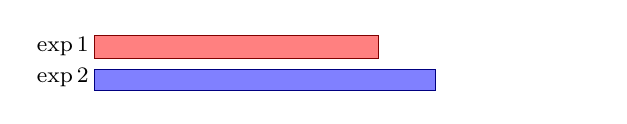
\begin{tikzpicture}[scale=0.4]
	\draw[color=white] (-2, -3) -- (16, -3);
	\node[font=\footnotesize] (e1) at (-1, -3.3) {$\exp{1}$};
	\node[font=\footnotesize] (e2) at (-1, -4.3) {$\exp{2}$};
	\filldraw[fill=red!50!white, draw=red!50!black] (0, -3.7) rectangle (9.02554, -2.9623);
	\filldraw[fill=blue!50!white, draw=blue!50!black] (0, -4.7) rectangle (10.8307, -4.04426);
\end{tikzpicture}
\end{center}
}

%\vspace{.05cm}

\uncover<3->{
\begin{center}
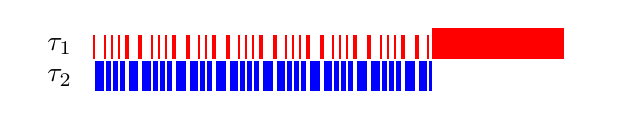
\begin{tikzpicture}[scale=0.4]
		\draw[color=white] (-2, -1) -- (16, -1);
% \draw[->] (-.2, -3.2) -- (15.2, -3.2) node[right] {time};
\node[] (t1) at (-1, -1.3) {$\tau_1$};
\node[] (t1) at (-1, -2.3) {$\tau_2$};
\fill[red] (0.0665893, -1.7) rectangle (0.130345, -0.929508);
\fill[blue] (0.130345, -2.7) rectangle (0.393197, -1.76557);
\fill[red] (0.393197, -1.7) rectangle (0.456953, -0.929508);
\fill[blue] (0.456953, -2.7) rectangle (0.614665, -1.76557);
\fill[red] (0.614665, -1.7) rectangle (0.67842, -0.929508);
\fill[blue] (0.67842, -2.7) rectangle (0.836132, -1.76557);
\fill[red] (0.836132, -1.7) rectangle (0.899887, -0.929508);
\fill[blue] (0.899887, -2.7) rectangle (1.0576, -1.76557);
\fill[red] (1.0576, -1.7) rectangle (1.18511, -0.929508);
\fill[blue] (1.18511, -2.7) rectangle (1.50053, -1.76557);
\fill[red] (1.50053, -1.7) rectangle (1.62804, -0.929508);
\fill[blue] (1.62804, -2.7) rectangle (1.8909, -1.76557);
\fill[red] (1.8909, -1.7) rectangle (1.95465, -0.929508);
\fill[blue] (1.95465, -2.7) rectangle (2.11236, -1.76557);
\fill[red] (2.11236, -1.7) rectangle (2.17612, -0.929508);
\fill[blue] (2.17612, -2.7) rectangle (2.33383, -1.76557);
\fill[red] (2.33383, -1.7) rectangle (2.39759, -0.929508);
\fill[blue] (2.39759, -2.7) rectangle (2.5553, -1.76557);
\fill[red] (2.5553, -1.7) rectangle (2.68281, -0.929508);
\fill[blue] (2.68281, -2.7) rectangle (2.99823, -1.76557);
\fill[red] (2.99823, -1.7) rectangle (3.12574, -0.929508);
\fill[blue] (3.12574, -2.7) rectangle (3.3886, -1.76557);
\fill[red] (3.3886, -1.7) rectangle (3.45235, -0.929508);
\fill[blue] (3.45235, -2.7) rectangle (3.61006, -1.76557);
\fill[red] (3.61006, -1.7) rectangle (3.67382, -0.929508);
\fill[blue] (3.67382, -2.7) rectangle (3.83153, -1.76557);
\fill[red] (3.83153, -1.7) rectangle (3.95904, -0.929508);
\fill[blue] (3.95904, -2.7) rectangle (4.27447, -1.76557);
\fill[red] (4.27447, -1.7) rectangle (4.40198, -0.929508);
\fill[blue] (4.40198, -2.7) rectangle (4.66483, -1.76557);
\fill[red] (4.66483, -1.7) rectangle (4.72858, -0.929508);
\fill[blue] (4.72858, -2.7) rectangle (4.8863, -1.76557);
\fill[red] (4.8863, -1.7) rectangle (4.95005, -0.929508);
\fill[blue] (4.95005, -2.7) rectangle (5.10776, -1.76557);
\fill[red] (5.10776, -1.7) rectangle (5.17152, -0.929508);
\fill[blue] (5.17152, -2.7) rectangle (5.32923, -1.76557);
\fill[red] (5.32923, -1.7) rectangle (5.45674, -0.929508);
\fill[blue] (5.45674, -2.7) rectangle (5.77216, -1.76557);
\fill[red] (5.77216, -1.7) rectangle (5.89968, -0.929508);
\fill[blue] (5.89968, -2.7) rectangle (6.16253, -1.76557);
\fill[red] (6.16253, -1.7) rectangle (6.22628, -0.929508);
\fill[blue] (6.22628, -2.7) rectangle (6.384, -1.76557);
\fill[red] (6.384, -1.7) rectangle (6.44775, -0.929508);
\fill[blue] (6.44775, -2.7) rectangle (6.60546, -1.76557);
\fill[red] (6.60546, -1.7) rectangle (6.66922, -0.929508);
\fill[blue] (6.66922, -2.7) rectangle (6.82693, -1.76557);
\fill[red] (6.82693, -1.7) rectangle (6.95444, -0.929508);
\fill[blue] (6.95444, -2.7) rectangle (7.26986, -1.76557);
\fill[red] (7.26986, -1.7) rectangle (7.39738, -0.929508);
\fill[blue] (7.39738, -2.7) rectangle (7.66023, -1.76557);
\fill[red] (7.66023, -1.7) rectangle (7.72398, -0.929508);
\fill[blue] (7.72398, -2.7) rectangle (7.8817, -1.76557);
\fill[red] (7.8817, -1.7) rectangle (7.94545, -0.929508);
\fill[blue] (7.94545, -2.7) rectangle (8.10316, -1.76557);
\fill[red] (8.10316, -1.7) rectangle (8.16692, -0.929508);
\fill[blue] (8.16692, -2.7) rectangle (8.32463, -1.76557);
\fill[red] (8.32463, -1.7) rectangle (8.45214, -0.929508);
\fill[blue] (8.45214, -2.7) rectangle (8.76756, -1.76557);
\fill[red] (8.76756, -1.7) rectangle (8.89508, -0.929508);
\fill[blue] (8.89508, -2.7) rectangle (9.15793, -1.76557);
\fill[red] (9.15793, -1.7) rectangle (9.22168, -0.929508);
\fill[blue] (9.22168, -2.7) rectangle (9.3794, -1.76557);
\fill[red] (9.3794, -1.7) rectangle (9.44315, -0.929508);
\fill[blue] (9.44315, -2.7) rectangle (9.60086, -1.76557);
\fill[red] (9.60086, -1.7) rectangle (9.66462, -0.929508);
\fill[blue] (9.66462, -2.7) rectangle (9.82233, -1.76557);
\fill[red] (9.82233, -1.7) rectangle (9.94984, -0.929508);
\fill[blue] (9.94984, -2.7) rectangle (10.2653, -1.76557);
\fill[red] (10.2653, -1.7) rectangle (10.3928, -0.929508);
\fill[blue] (10.3928, -2.7) rectangle (10.6556, -1.76557);
\fill[red] (10.6556, -1.7) rectangle (10.7194, -0.929508);
\fill[blue] (10.7194, -2.7) rectangle (10.8245, -1.76557);
\fill[red] (10.8245, -1.7) rectangle (15, -0.7);
\end{tikzpicture}
\end{center}
}



%\vspace{.05cm}

\uncover<4->{
\begin{center}
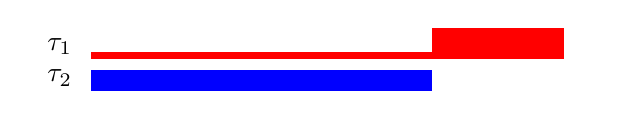
\begin{tikzpicture}[scale=0.4]
		\draw[color=white] (-2, -1) -- (16, -1);
% \draw[color=red, line width=2pt] (0,0) edge (9.02554,1.66572);
% \draw[color=red, line width=2pt] (9.02554,1.66572) edge (10.8307,1.515);
% \draw[color=red, line width=2pt] (10.8307,1.515) edge (15,0);
% \draw[color=blue, line width=2pt] (0,0) edge (9.02554,0);
% \draw[color=blue, line width=2pt] (9.02554,0) edge (10.8307,0);
% \draw[color=blue, line width=2pt] (10.8307,0) edge (15,0);
% \draw[color=black, line width=2pt] (0,0) edge (9.02554,2.90417);
% \draw[color=black, line width=2pt] (9.02554,2.90417) edge (10.8307,3.485);
% \draw[color=black, line width=2pt] (10.8307,3.485) edge (15,5);
\node[] (t1) at (-1, -1.3) {$\tau_1$};
\node[] (t1) at (-1, -2.3) {$\tau_2$};
% \draw[] (15.2, 5.2) node[right] {$m_m$};
% \draw[->] (-.2, -.2) -- (15.2, -.2) node[right] {time};
% \draw[->] (-.2, -.2) -- (-.2, 5.2) node[right] {memory};
% \draw[step=35.8423,very thin,color=gray] (0,0) grid (15, 5);
\fill[blue] (0, -2.7) rectangle (9.02554, -2.04426);
\fill[red] (0, -1.7) rectangle (9.02554, -1.4702);
\fill[blue] (9.02554, -2.7) rectangle (10.8307, -2.04426);
\fill[red] (9.02554, -1.7) rectangle (10.8307, -1.4702);
\fill[red] (10.8307, -1.7) rectangle (15, -0.7);
\end{tikzpicture}
\end{center}
}

\end{columns}


\end{frame}


\begin{frame}[fragile]
	\frametitle{Checking the Constraint}

\begin{center}
\begin{tikzpicture}[scale = 0.55]


%\draw (8.6353, -6.5) rectangle (15, -1);




\filldraw[fill=red!50!white, draw=red!50!black] (0, -4) rectangle (1.68224, -3.85714);
\filldraw[fill=green!50!white, draw=green!50!black] (0.841121, -6) rectangle (2.24299, -5.08571);
\filldraw[fill=red!50!white, draw=red!50!black] (4.48598, -4) rectangle (6.72897, -3.85714);
\filldraw[fill=blue!50!white, draw=blue!50!black] (5.04673, -5) rectangle (8.41121, -4.46429);
\filldraw[fill=green!50!white, draw=green!50!black] (7.85047, -6) rectangle (10.0935, -5.10714);
\filldraw[fill=red!50!white, draw=red!50!black] (7.57009, -4) rectangle (10.3738, -3.85714);
\filldraw[fill=blue!50!white, draw=blue!50!black] (9.25234, -5) rectangle (12.0561, -4.57143);
\filldraw[fill=green!50!white, draw=green!50!black] (11.215, -6) rectangle (12.6168, -5.08571);

\draw[->] (-.2, -.2) -- (15.2, -.2) node[right] {{\footnotesize time}};
\draw[->] (-.2, -.2) -- (-.2, 5.2) node[right] {{\footnotesize memory}};
\draw[step=46.9484,very thin,color=gray] (0,0) grid (15, 5);


\node[] (e1) at (-1, -4) {\scriptsize{$\exp{1}$}};
\node[] (e2) at (-1, -4.7) {\scriptsize{$\exp{2}$}};
\node[] (e3) at (-1, -5.6) {\scriptsize{$\exp{3}$}};


\uncover<1-> {


\node[] (t1) at (-1, -1.5) {\scriptsize{$\tau_1$}};

\draw[color=black, line width=1.5pt] (0,0) edge (0.841121,0.0704225);
\draw[color=green, line width=1.5pt] (0,0) edge (0.841121,0);
\draw[color=blue, line width=1.5pt] (0,0) edge (0.841121,0);
\draw[color=red, line width=1.5pt] (0,0) edge (0.841121,0);
\fill[red] (0, -1.7) rectangle (0.841121, -1.53607);
\only<1-3> \draw[dashed] (0.841121, -1) -- (0.841121, -6.5);

}
\uncover<2-> {


\node[] (t3) at (-1, -3.2) {\scriptsize{$\tau_3$}};

\draw[color=black, line width=1.5pt] (0.841121,0.0704225) edge (1.68224,0.413763);
\draw[color=green, line width=1.5pt] (0.841121,0) edge (1.68224,0.177786);
\draw[color=blue, line width=1.5pt] (0.841121,0) edge (1.68224,0);
\draw[color=red, line width=1.5pt] (0.841121,0) edge (1.68224,0);
\fill[red] (0.841121, -1.7) rectangle (1.68224, -1.53607);
\fill[green] (0.841121, -3.7) rectangle (1.68224, -3.06468);
\only<2-4> \draw[dashed] (1.68224, -1) -- (1.68224, -6.5);

}
\uncover<3-> {

\draw[color=black, line width=1.5pt] (1.68224,0.413763) edge (2.24299,0.634421);
\draw[color=green, line width=1.5pt] (1.68224,0.177786) edge (2.24299,0.257598);
\draw[color=blue, line width=1.5pt] (1.68224,0) edge (2.24299,0);
\draw[color=red, line width=1.5pt] (1.68224,0) edge (2.24299,0);
\fill[green] (1.68224, -3.7) rectangle (2.24299, -2.92951);
\only<3-5> \draw[dashed] (2.24299, -1) -- (2.24299, -6.5);

}
\uncover<4-> {

\draw[color=black, line width=1.5pt] (2.24299,0.634421) edge (2.89761,0.892019);
\draw[color=green, line width=1.5pt] (2.24299,0.257598) edge (2.89761,0);
\draw[color=blue, line width=1.5pt] (2.24299,0) edge (2.89761,0);
\draw[color=red, line width=1.5pt] (2.24299,0) edge (2.89761,0);
\fill[green] (2.24299, -3.7) rectangle (2.89761, -2.92951);
\only<4-6> \draw[dashed] (2.89761, -1) -- (2.89761, -6.5);

}
\uncover<5-> {

\draw[color=black, line width=1.5pt] (2.89761,0.892019) edge (4.48598,0.892019);
\draw[color=green, line width=1.5pt] (2.89761,0) edge (4.48598,0);
\draw[color=blue, line width=1.5pt] (2.89761,0) edge (4.48598,0);
\draw[color=red, line width=1.5pt] (2.89761,0) edge (4.48598,0);
\only<5-7> \draw[dashed] (4.48598, -1) -- (4.48598, -6.5);

}
\uncover<6-> {

\draw[color=black, line width=1.5pt] (4.48598,0.892019) edge (5.04673,0.938967);
\draw[color=green, line width=1.5pt] (4.48598,0) edge (5.04673,0);
\draw[color=blue, line width=1.5pt] (4.48598,0) edge (5.04673,0);
\draw[color=red, line width=1.5pt] (4.48598,0) edge (5.04673,0);
\fill[red] (4.48598, -1.7) rectangle (5.04673, -1.53607);
\only<6-8> \draw[dashed] (5.04673, -1) -- (5.04673, -6.5);

}
\uncover<7-> { 

\node[] (t2) at (-1, -2.4) {\scriptsize{$\tau_2$}};

\draw[color=black, line width=1.5pt] (5.04673,0.938967) edge (6.72897,1.5455);
\draw[color=green, line width=1.5pt] (5.04673,0) edge (6.72897,0);
\draw[color=blue, line width=1.5pt] (5.04673,0) edge (6.72897,0.0624813);
\draw[color=red, line width=1.5pt] (5.04673,0) edge (6.72897,0);
\fill[red] (5.04673, -1.7) rectangle (6.72897, -1.53607);
\fill[blue] (5.04673, -2.7) rectangle (6.72897, -2.15797);
\only<7-9> \draw[dashed] (6.72897, -1) -- (6.72897, -6.5);


}
\uncover<8-> {

\draw[color=black, line width=1.5pt] (6.72897,1.5455) edge (7.57009,1.84127);
\draw[color=green, line width=1.5pt] (6.72897,0) edge (7.57009,0);
\draw[color=blue, line width=1.5pt] (6.72897,0.0624813) edge (7.57009,0.0307911);
\draw[color=red, line width=1.5pt] (6.72897,0) edge (7.57009,0);
\fill[blue] (6.72897, -2.7) rectangle (7.57009, -2.01148);
\only<8-10> \draw[dashed] (7.57009, -1) -- (7.57009, -6.5);

}
\uncover<9-> {

\draw[color=black, line width=1.5pt] (7.57009,1.84127) edge (7.85047,1.94236);
\draw[color=green, line width=1.5pt] (7.57009,0) edge (7.85047,0);
\draw[color=blue, line width=1.5pt] (7.57009,0.0307911) edge (7.85047,0.0412047);
\draw[color=red, line width=1.5pt] (7.57009,0) edge (7.85047,0);
\fill[red] (7.57009, -1.7) rectangle (7.85047, -1.53607);
\fill[blue] (7.57009, -2.7) rectangle (7.85047, -2.15797);
\only<9-11> \draw[dashed] (7.85047, -1) -- (7.85047, -6.5);

}
\uncover<10-> {

\draw[color=black, line width=1.5pt] (7.85047,1.94236) edge (8.41121,2.14454);
\draw[color=green, line width=1.5pt] (7.85047,0) edge (8.41121,0.293427);
\draw[color=blue, line width=1.5pt] (7.85047,0.0412047) edge (8.41121,0.0620318);
\draw[color=red, line width=1.5pt] (7.85047,0) edge (8.41121,0);
\fill[red] (7.85047, -1.7) rectangle (8.41121, -1.53607);
\fill[blue] (7.85047, -2.7) rectangle (8.41121, -2.15797);
\only<10-12> \draw[dashed] (8.41121, -1) -- (8.41121, -6.5);

}
\uncover<11-> {

\draw[color=black, line width=1.5pt] (8.41121,2.14454) edge (8.6353,2.22533);
\draw[color=green, line width=1.5pt] (8.41121,0.293427) edge (8.6353,0.410685);
\draw[color=blue, line width=1.5pt] (8.41121,0.0620318) edge (8.6353,0);
\draw[color=red, line width=1.5pt] (8.41121,0) edge (8.6353,0);
\fill[red] (8.41121, -1.7) rectangle (8.6353, -1.53607);
\fill[blue] (8.41121, -2.7) rectangle (8.6353, -2.15797);
\only<11-13> \draw[dashed] (8.6353, -1) -- (8.6353, -6.5);

}
\uncover<12-> {

\draw[color=black, line width=1.5pt] (8.6353,2.22533) edge (9.25234,2.43154);
\draw[color=green, line width=1.5pt] (8.6353,0.410685) edge (9.25234,0.579024);
\draw[color=blue, line width=1.5pt] (8.6353,0) edge (9.25234,0);
\draw[color=red, line width=1.5pt] (8.6353,0) edge (9.25234,0);
\fill[red] (8.6353, -1.7) rectangle (9.25234, -1.53607);
\fill[green] (8.6353, -3.7) rectangle (9.25234, -3.20959);
\only<12-14> \draw[dashed] (9.25234, -1) -- (9.25234, -6.5);

}
\uncover<13-> {

\draw[color=black, line width=1.5pt] (9.25234,2.43154) edge (10.0935,2.73275);
\draw[color=green, line width=1.5pt] (9.25234,0.579024) edge (10.0935,0.999643);
\draw[color=blue, line width=1.5pt] (9.25234,0) edge (10.0935,0);
\draw[color=red, line width=1.5pt] (9.25234,0) edge (10.0935,0);
\fill[red] (9.25234, -1.7) rectangle (10.0935, -1.53607);
\fill[blue] (9.25234, -2.7) rectangle (10.0935, -2.2082);
\fill[green] (9.25234, -3.7) rectangle (10.0935, -3.65456);
\only<13-15> \draw[dashed] (10.0935, -1) -- (10.0935, -6.5);

}
\uncover<14-> {

\draw[color=black, line width=1.5pt] (10.0935,2.73275) edge (10.3738,2.83315);
\draw[color=green, line width=1.5pt] (10.0935,0.999643) edge (10.3738,0.993136);
\draw[color=blue, line width=1.5pt] (10.0935,0) edge (10.3738,0);
\draw[color=red, line width=1.5pt] (10.0935,0) edge (10.3738,0);
\fill[red] (10.0935, -1.7) rectangle (10.3738, -1.53607);
\fill[blue] (10.0935, -2.7) rectangle (10.3738, -2.2082);
\fill[green] (10.0935, -3.7) rectangle (10.3738, -3.65456);
\only<14-16> \draw[dashed] (10.3738, -1) -- (10.3738, -6.5);

}
\uncover<15-> {

\draw[color=black, line width=1.5pt] (10.3738,2.83315) edge (11.215,3.20121);
\draw[color=green, line width=1.5pt] (10.3738,0.993136) edge (11.215,0.836353);
\draw[color=blue, line width=1.5pt] (10.3738,0) edge (11.215,0);
\draw[color=red, line width=1.5pt] (10.3738,0) edge (11.215,0);
\fill[blue] (10.3738, -2.7) rectangle (11.215, -2.2082);
\fill[green] (10.3738, -3.7) rectangle (11.215, -3.33503);
\only<15-17> \draw[dashed] (11.215, -1) -- (11.215, -6.5);

}
\uncover<16-> {

\draw[color=black, line width=1.5pt] (11.215,3.20121) edge (12.0561,3.56926);
\draw[color=green, line width=1.5pt] (11.215,0.836353) edge (12.0561,1.13027);
\draw[color=blue, line width=1.5pt] (11.215,0) edge (12.0561,0);
\draw[color=red, line width=1.5pt] (11.215,0) edge (12.0561,0);
\fill[blue] (11.215, -2.7) rectangle (12.0561, -2.2082);
\fill[green] (11.215, -3.7) rectangle (12.0561, -3.33503);
\only<16-18> \draw[dashed] (12.0561, -1) -- (12.0561, -6.5);

}
\uncover<17-> {

\draw[color=black, line width=1.5pt] (12.0561,3.56926) edge (12.6168,3.85564);
\draw[color=black, line width=1.5pt] (12.6168,3.85564) edge (14.8575,5);
\draw[color=green, line width=1.5pt] (12.0561,1.13027) edge (12.6168,1.14436);
\draw[color=green, line width=1.5pt] (12.6168,1.14436) edge (14.8575,0);
\draw[color=blue, line width=1.5pt] (12.0561,0) edge (12.6168,0);
\draw[color=blue, line width=1.5pt] (12.6168,0) edge (14.8575,0);
\draw[color=red, line width=1.5pt] (12.0561,0) edge (12.6168,0);
\draw[color=red, line width=1.5pt] (12.6168,0) edge (14.8575,0);
\fill[green] (12.0561, -3.7) rectangle (14.8575, -2.7);

}

\end{tikzpicture}
\end{center}
% \uncover<5->{
% \begin{itemize}
% 	\item We can jump from \memph{"event"} to \memph{"event"}: \memph{$O(n \log n)$} worst case time complexity
% \end{itemize}
% }

\end{frame}



\begin{frame}[fragile]
  \frametitle{Sweep algorithm~\mycite{BeldiceanuCarlsson01}}
    
		\begin{itemize}
			\item The constraint can be checked in $\memph{O(n \log n)}$
			\pause \item Several experiments active simultaneously:
			\begin{itemize}
				\item Error is less than or equal to \memph{$1 + \frac{\tau^{max}}{\tau^{min}} \simeq 3$} blocks \\~
			\end{itemize}			
			\pause \item \memph{Faster and more accurate than the reservoir/transfer tasks model}
			
			\pause \item Bound adjustments? Two principles:
			\begin{itemize}
				\item Producing too much data too quickly can lead to data loss
				\item Filling up the mass memory while not in visibility can lead to data loss
			\end{itemize}
		\end{itemize}
	
\end{frame}


	\def\tsat{\overline{t}}


\begin{frame}[fragile]
\frametitle{Propagation: production/transfer rate}
\begin{myblock}{For a set of tasks}
\begin{itemize}
\item \memph{lower bound} on how much time the CDMS needs to transfer without data loss
\end{itemize}
\end{myblock}

\medskip

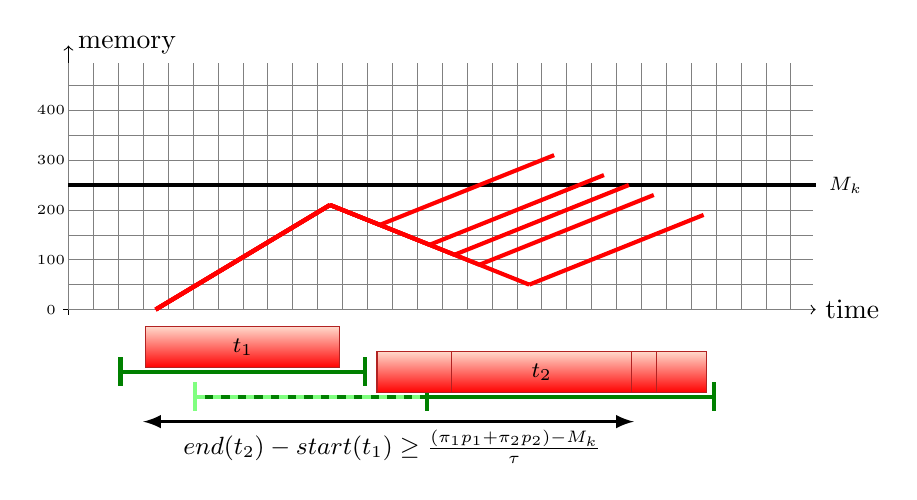
\begin{tikzpicture}[scale=0.9]
	
\tikzset{task/.style={draw=FireBrick,top color=OrangeRed!20, bottom color=Red, minimum height=15pt, shape=rectangle, font=\footnotesize}}
\tikzset{t1/.style={task, minimum width=70pt}}
\tikzset{t2/.style={task, minimum width=65pt}}
	
\node[t1] (t31) at (70pt,-15pt) {$t_1$};
\draw[|-|, ultra thick, green!50!black] (20pt,-25pt) -- (120pt,-25pt);

\uncover<1-4> {
\draw[|-|, ultra thick, green!50!black] (50pt,-35pt) -- (260pt,-35pt);
}

\uncover<5> {
\draw[|-, dashed, ultra thick, green!50] (50pt,-35pt) -- (143pt,-35pt);
\draw[|-|, ultra thick, green!50!black] (143pt,-35pt) -- (260pt,-35pt);
}

\draw[->] (-2pt,0pt) -- (300pt,0pt) node[right] {time};
\draw[->] (0pt,-2pt) -- (0pt,106pt) node[right] {memory};
\draw[step=10pt,very thin,color=gray] (0pt,0pt) grid (299pt,99pt);
\node[] (mark0) at (-7pt,0pt) {{\tiny 0}};
\node[] (mark20) at (-7pt,20pt) {{\tiny 100}};
\node[] (mark40) at (-7pt,40pt) {{\tiny 200}};
\node[] (mark60) at (-7pt,60pt) {{\tiny 300}};
\node[] (mark80) at (-7pt,80pt) {{\tiny 400}};

\draw[color=black, line width=1.5pt] (0pt,50pt) edge (300pt,50pt);
\node[] (mark0) at (312pt,50pt) {{\scriptsize $M_k$}};

\uncover<1>{
\node[t2] (t32) at (220pt,-25pt) {$t_2$};
\draw[color=red, line width=1.5pt] (35pt,0pt) edge (105pt,42pt);
\draw[color=red, line width=1.5pt] (105pt,42pt) edge (185pt,10pt);
\draw[color=red, line width=1.5pt] (185pt,10pt) edge (255pt,38pt);
}

\uncover<2>{
\node[t2] (t32) at (200pt,-25pt) {$t_2$};
\draw[color=red, line width=1.5pt] (35pt,0pt) edge (105pt,42pt);
\draw[color=red, line width=1.5pt] (105pt,42pt) edge (165pt,18pt);
\draw[color=red, line width=1.5pt] (165pt,18pt) edge (235pt,46pt);
}

\uncover<3>{
\node[t2] (t32) at (180pt,-25pt) {$t_2$};
\draw[color=red, line width=1.5pt] (35pt,0pt) edge (105pt,42pt);
\draw[color=red, line width=1.5pt] (105pt,42pt) edge (145pt,26pt);
\draw[color=red, line width=1.5pt] (145pt,26pt) edge (215pt,54pt);
}

\uncover<4>{
\node[t2] (t32) at (160pt,-25pt) {$t_2$};
\draw[color=red, line width=1.5pt] (35pt,0pt) edge (105pt,42pt);
\draw[color=red, line width=1.5pt] (105pt,42pt) edge (125pt,34pt);
\draw[color=red, line width=1.5pt] (125pt,34pt) edge (195pt,62pt);
}


\uncover<5>{
\node[t2] (t32) at (190pt,-25pt) {$t_2$};
\draw[color=red, line width=1.5pt] (35pt,0pt) edge (105pt,42pt);
\draw[color=red, line width=1.5pt] (105pt,42pt) edge (155pt,22pt);
\draw[color=red, line width=1.5pt] (155pt,22pt) edge (225pt,50pt);

\draw[latex-latex, very thick] (30pt,-45pt) -- (227pt,-45pt);
\node[] (mark0) at (130pt,-55pt) {{\small \memph{$end(t_2) - start(t_1) \geq \frac{(\pi_1 p_1 + \pi_2 p_2)-M_k}{\tau}$}}};
}


\end{tikzpicture}

\end{frame}


\begin{frame}
	\frametitle{Propagation: production/transfer rate}
	
	More generally, we consider a set of tasks \memph{$\Omega$} of a given experiment
	\begin{itemize}
		%\item Let \memph{$[a,b]=[\min_{t_{ki}\in \Omega}(\max(s_{ki})), \max_{t_{ki}\in \Omega}(\min(s_{ki}+p_{ki}))]$}
		\pause \item Let \memph{$[a,b]$} be a time interval \memph{necessarily} contained in \memph{$\Omega$}'s transfer period 
		\pause \item We can take into account the tasks of higher priority producing during \memph{$[a,b]$}
	\end{itemize}
	
\pause \begin{myblock}{Filtering rule}
\begin{itemize}
%\item Let \memph{$min(|t_{ki}\cap[a,b]|)$} be the minimal intersection between \memph{$t_{ki}$} and \memph{$[a,b]$}
\item 
Minimum amount of higher priority data to transfer on \memph{$[a,b]$} over transfer rate:
\begin{itemize}
	\item Lower bound on the time dedicated to higher priority experiment: \memph{$T_k(a,b)$}
\end{itemize}
% \begin{itemize}
% 	\item \memph{$\sum_{j=1}^{j<R(k)} \sum_{i=1}^n \min(|t_{P(j)i} \cap [a,b]|)*\pi_{P(j)i}$}
% \end{itemize}
% \pause
% \item Necessary duration:\\
% \hspace{1cm} \memph{$T_k(a,b)= \dfrac{\sum_{j=1}^{j<R(k)} \sum_{i=1}^n \min(|t_{P(j)i} \cap [a,b]|)*\pi_{P(j)i}}{\tau}$}
\pause 
\item Induced constraint:\\
\hspace{1cm} \memph{$Makespan(\Omega) \geq \frac{(\sum_{t_{ki}\in \Omega} \pi_i p_i)-M_k}{\tau} + T_k(a,b)$}
%\memph{$\max_{t_{ki} \in \Omega}(e_{ki}) - \min_{t_{ki} \in \Omega}(s_{ki}) \geq \frac{(\sum_{t_{ki}\in \Omega} \pi_i p_i)-M_k}{\tau} + T_k(a,b)$}

\end{itemize}
\end{myblock}

\end{frame}

	
	
\begin{frame}
  \frametitle{Propagation: visibility}
  
	
	\begin{itemize}
		\item When the mass memory is full, no more data is transferred to it
		\uncover<2->{\item Minimal usage and peak \memph{$m_0^{max}$}
%		\item Compute the date \memph{$\tsat$} at which the usage reaches its maximum \memph{$m_0^{\tsat}$}
		\uncover<3->{%\item Given an experiment with memory \memph{$M_k$}
		%\begin{itemize}
			\item If the production exceeds \memph{$M_k + M_0 - m_0^{max}$} in \memph{$[a, b]$} then data will be \memph{lost}
		%\end{itemize}
		\uncover<4->{
		\begin{itemize}
			\item \memph{Filtering: bound start time w.r.t. this quantity of data and production rate}
		\end{itemize}
		}
		}
		}
	\end{itemize}


\begin{center}
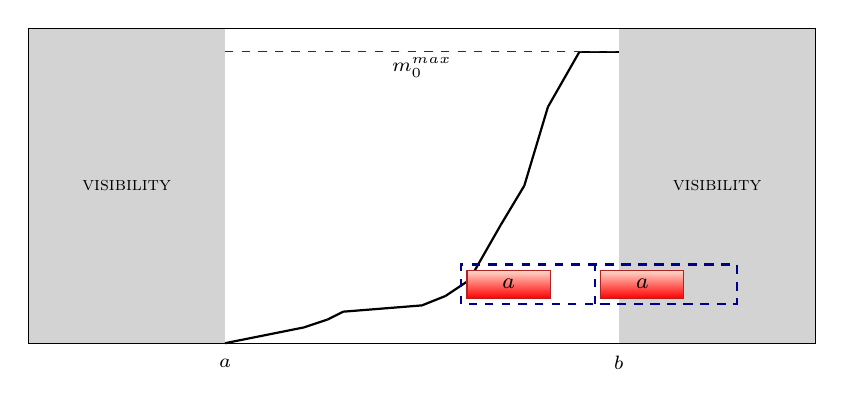
\begin{tikzpicture}
	
	\tikzset{task/.style={draw=FireBrick,top color=OrangeRed!20, bottom color=Red, minimum height=10pt, shape=rectangle, font=\footnotesize, minimum width=30pt}}
	
		 
		 \fill[color=LightGray] (0,0) rectangle (2.5,4);
		 \node[font=\scriptsize] at (1.25,2) {{\sc visibility}};
		 \fill[color=LightGray] (7.5,0) rectangle (10,4);
		 \node[font=\scriptsize] at (8.75,2) {{\sc visibility}};
		 \draw[color=black] (0,0) rectangle (10,4);
		 
		 \uncover<2-> {
		 \draw[thick] (2.5,0) -- (3.5,.2);
		 \draw[thick] (3.5,.2) -- (3.8,.3);
		 \draw[thick] (3.8,.3) -- (4,.4);
		 \draw[thick] (4,.4) -- (5,.48);
		 \draw[thick] (5,.48) -- (5.3,.6);
		 \draw[thick] (5.3,.6) -- (5.6,.8);
		 \draw[thick] (5.6,.8) -- (6,1.5);
		 \draw[thick] (6,1.5) -- (6.3,2);
		 \draw[thick] (6.3,2) -- (6.6,3);
		 \draw[thick] (6.6,3) -- (7,3.7);
		 \draw[thick] (7,3.7) -- (7.5,3.7);
		 
		 %\draw[dashed, color=red!60!black] (7,0) -- (7,4);
		 
		 \draw[dashed, color=red!60!black] (2.5,3.7) -- (7.5,3.7);
		 
%		 \node[font=\scriptsize] at (7, -.2) {$\tsat$};
		 \node[font=\scriptsize] at (2.5, -.25) {$a$};
		 \node[font=\scriptsize] at (7.5, -.25) {$b$};
		 \node[font=\scriptsize] at (5, 3.5) {\memph{$m_0^{max}$}};
		 }
		 
		 
		 \uncover<3> {
		 \draw[dashed, color=DarkBlue, thick] (5.5,.5) rectangle (9,1);
		 \node[task] at (6.1,.75) {$a$};
		 }
		 
		 \uncover<4> {
		 \draw[dashed, color=DarkBlue, thick] (7.2,.5) rectangle (9,1);
		 \node[task] at (7.8,.75) {$a$};
		 }
		 
				 
\end{tikzpicture}
\end{center}


\end{frame}















